\section{What combinatorics studies}

Combinatorics is the mathematics of counting possibilities. In this chapter we study how to count arrangements, selections, and structured lists of objects.

The main question is simple to state:
\[
\text{How many objects of a given type can be formed?}
\]
The answer depends on the rules. Does order matter? Can an object be used more than once? Do we use all objects, or only some of them? These questions lead to different counting schemes.

We will use six basic schemes:
\[
\begin{array}{c|c|c}
\text{scheme} & \text{order matters?} & \text{repetition allowed?} \\
\hline
\text{permutations without repetition} & \text{yes} & \text{no} \\
\text{permutations with repetition} & \text{yes} & \text{yes, through identical objects} \\
\text{variations without repetition} & \text{yes} & \text{no} \\
\text{variations with repetition} & \text{yes} & \text{yes} \\
\text{combinations without repetition} & \text{no} & \text{no} \\
\text{combinations with repetition} & \text{no} & \text{yes}
\end{array}
\]

The goal of the chapter is not only to memorize formulas. The goal is to recognize the structure of a counting problem.

\section{Permutations without repetition}

Combinatorics begins with arrangements. Imagine a row of empty places and a collection of distinct objects. We want to fill all places, using every object exactly once. In this situation, changing the order changes the result.

This is the most basic ordered counting scheme. It appears whenever the question is about arranging, ranking, scheduling, ordering, or placing all available distinct objects in a line.

\begin{definitionbox}
Let \(A\) be a finite set with \(n\) distinct elements. A permutation without repetition of the elements of \(A\) is an ordering of all elements of \(A\), in which every element appears exactly once.
\end{definitionbox}

For example, if
\[
A=\{a,b,c\},
\]
then the permutations without repetition are
\[
abc,\quad acb,\quad bac,\quad bca,\quad cab,\quad cba.
\]
There are six of them.

\begin{center}
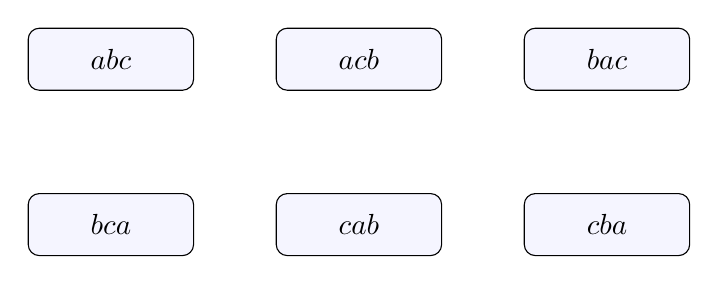
\begin{tikzpicture}[scale=1.05, transform shape]
\foreach \word/\x/\y in {abc/0/2, acb/3/2, bac/6/2, bca/0/0, cab/3/0, cba/6/0} {
    \node[draw, rounded corners, fill=blue!4, minimum width=2.0cm, minimum height=0.75cm] at (\x,\y) {$\word$};
}
\end{tikzpicture}
\end{center}

\begin{theorembox}
The number of permutations without repetition of \(n\) distinct elements is
\[
n! = n(n-1)(n-2)\cdots 2\cdot 1.
\]
\end{theorembox}

The formula follows directly from the multiplication principle. There are \(n\) choices for the first place. Once the first object has been used, there are only \(n-1\) choices for the second place. After two objects have been used, there are \(n-2\) choices for the third place. Continuing this reasoning gives
\[
n(n-1)(n-2)\cdots 2\cdot 1=n!.
\]

The decreasing number of choices is the signature of ``without repetition''. Each decision removes one object from later use.

\begin{examplebox}
Five different books are to be arranged on a shelf. Since all books are used, all books are distinct, and order matters, this is a permutation without repetition. The number of possible arrangements is
\[
5!=5\cdot4\cdot3\cdot2\cdot1=120.
\]
\end{examplebox}

\begin{examplebox}
Four students are to stand in a single line for a photograph. The students are distinct, every student stands in the line, and changing the order gives a different line. The number of possible lines is
\[
4!=24.
\]
\end{examplebox}

\begin{remarkbox}
Use permutations without repetition when all objects are distinct, all objects are used, and order matters. Typical words are: arrange, order, rank, line up, schedule all, place all.
\end{remarkbox}

\section{Permutations with repetition}

Permutations without repetition assume that all objects are distinct. In many counting problems this is not true. Some objects may look the same, carry the same label, or belong to the same type. Then exchanging two identical objects does not create a new visible arrangement.

The important idea is overcounting. If we temporarily pretend that all objects are distinct, we count too many arrangements. We then divide by the number of internal swaps that cannot be seen in the final result.

\begin{definitionbox}
A permutation with repetition is an ordering of a multiset, that is, a finite collection in which some elements may occur more than once.
\end{definitionbox}

For example, the letters in the word
\[
AAB
\]
are not all distinct. The two letters \(A\) are indistinguishable. The distinct arrangements are
\[
AAB,\qquad ABA,\qquad BAA.
\]
There are three, not six.

If all three positions were occupied by distinct objects, there would be \(3!\) arrangements. But the two identical \(A\)'s can be swapped without producing a new visible arrangement. Therefore we divide by \(2!\).

\begin{theorembox}
Suppose a multiset has \(n\) elements in total, with \(n_1\) identical elements of one kind, \(n_2\) identical elements of another kind, and so on, where
\[
n_1+n_2+\cdots+n_k=n.
\]
The number of distinct permutations is
\[
\frac{n!}{n_1!n_2!\cdots n_k!}.
\]
\end{theorembox}

The numerator \(n!\) counts arrangements as if every object were distinct. The denominator removes invisible rearrangements inside each group of identical objects. If one kind appears \(n_i\) times, then those \(n_i\) identical copies can be internally rearranged in \(n_i!\) ways without changing the final visible arrangement.

\begin{examplebox}
How many distinct arrangements are there of the letters in the word \(\text{LEVEL}\)?

There are five letters. The letter \(L\) appears twice, the letter \(E\) appears twice, and the letter \(V\) appears once. Hence
\[
\frac{5!}{2!2!1!}=\frac{120}{4}=30.
\]
\end{examplebox}

\begin{examplebox}
How many distinct strings can be formed from the letters of \(\text{AABBC}\)?

There are five positions. The letter \(A\) appears twice, \(B\) appears twice, and \(C\) appears once. Therefore the number is
\[
\frac{5!}{2!2!1!}=30.
\]
\end{examplebox}

\begin{remarkbox}
Use permutations with repetition when all positions are filled, order matters, and some objects are indistinguishable. Typical examples are arrangements of letters in a word with repeated letters or arrangements of objects classified by type rather than identity.
\end{remarkbox}

\section{Variations without repetition}

A permutation uses all available objects. A variation uses only some of them. The order still matters, but we stop after filling \(k\) positions.

This situation appears when we form a short ordered list from a larger collection: a podium with first, second, and third place; a code made of different symbols; a sequence of selected objects; or an ordered assignment of distinct objects to distinct positions.

\begin{definitionbox}
Let \(A\) be a finite set with \(n\) distinct elements, and let \(k\leq n\). A variation without repetition of length \(k\) is an ordered selection of \(k\) distinct elements from \(A\).
\end{definitionbox}

For example, from
\[
A=\{a,b,c\}
\]
the variations without repetition of length \(2\) are
\[
ab,\quad ac,\quad ba,\quad bc,\quad ca,\quad cb.
\]
The selections \(ab\) and \(ba\) are different, because order matters.

\begin{center}
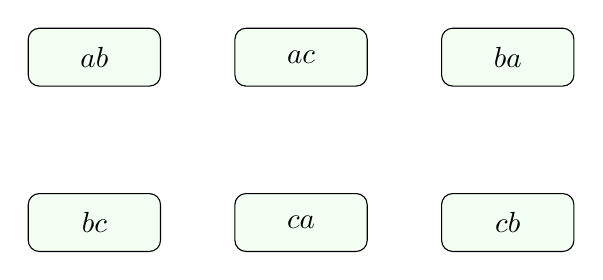
\begin{tikzpicture}[scale=1.05, transform shape]
\foreach \word/\x/\y in {ab/0/2, ac/2.5/2, ba/5/2, bc/0/0, ca/2.5/0, cb/5/0} {
    \node[draw, rounded corners, fill=green!5, minimum width=1.6cm, minimum height=0.7cm] at (\x,\y) {$\word$};
}
\end{tikzpicture}
\end{center}

\begin{theorembox}
The number of variations without repetition of length \(k\) chosen from \(n\) distinct elements is
\[
V(n,k)=n(n-1)(n-2)\cdots(n-k+1)=\frac{n!}{(n-k)!}.
\]
\end{theorembox}

There are \(n\) choices for the first position, \(n-1\) choices for the second position, and so on. Since no element may be repeated, the number of choices decreases after each position is filled. We stop after \(k\) positions, so the product has only \(k\) factors.

A useful mental picture is a row of \(k\) boxes:
\[
\boxed{\phantom{a}}\quad \boxed{\phantom{a}}\quad \cdots \quad \boxed{\phantom{a}}.
\]
The first box has \(n\) possible fillings, the second has \(n-1\), and the process continues until the \(k\)-th box.

\begin{examplebox}
A code consists of three different letters chosen from the six letters
\[
A,B,C,D,E,F.
\]
Order matters and no letter may repeat. The number of possible codes is
\[
V(6,3)=6\cdot5\cdot4=120.
\]
\end{examplebox}

\begin{examplebox}
Eight runners compete for three medals: gold, silver, and bronze. The order matters because the medals are different, and no runner can receive more than one medal. Thus the number of possible medal outcomes is
\[
V(8,3)=8\cdot7\cdot6=336.
\]
\end{examplebox}

\begin{remarkbox}
Use variations without repetition when order matters, only \(k\) positions are filled, and no object may be used more than once. This is the ordered-selection scheme.
\end{remarkbox}

\section{Variations with repetition}

In some ordered selections, the same object may be used more than once. Then the number of choices does not decrease from one position to the next.

\begin{definitionbox}
Let \(A\) be a finite set with \(n\) distinct elements. A variation with repetition of length \(k\) is an ordered \(k\)-tuple of elements of \(A\), where elements may repeat.
\end{definitionbox}

For example, if
\[
A=\{a,b\},
\]
then the variations with repetition of length \(3\) are
\[
aaa,\quad aab,\quad aba,\quad abb,\quad baa,\quad bab,\quad bba,\quad bbb.
\]
There are \(8\) of them.

\begin{theorembox}
The number of variations with repetition of length \(k\) chosen from \(n\) distinct elements is
\[
n^k.
\]
\end{theorembox}

There are \(n\) choices for the first position. Because repetition is allowed, there are again \(n\) choices for the second position, again \(n\) choices for the third position, and so on. Therefore the multiplication principle gives
\[
\underbrace{n\cdot n\cdots n}_{k\text{ factors}}=n^k.
\]

\begin{examplebox}
A three-symbol string is formed from the alphabet
\[
\{0,1,2,3,4,5,6,7,8,9\}.
\]
Symbols may repeat. There are
\[
10^3=1000
\]
such strings.
\end{examplebox}

\begin{remarkbox}
Use variations with repetition when order matters, there are \(k\) positions, and every position can be filled independently from the same set of \(n\) objects.
\end{remarkbox}

\section{Combinations without repetition}

In combinations, order does not matter. We are interested only in which objects are selected, not in the order in which they are written.

This is a different way of thinking from permutations and variations. In an ordered list, \(ab\) and \(ba\) are different. In an unordered selection, they represent the same choice. The objects are collected into a group, not placed into positions.

\begin{definitionbox}
Let \(A\) be a finite set with \(n\) distinct elements, and let \(k\leq n\). A combination without repetition of size \(k\) is a \(k\)-element subset of \(A\).
\end{definitionbox}

For example, if
\[
A=\{a,b,c\},
\]
then the combinations without repetition of size \(2\) are
\[
\{a,b\},\qquad \{a,c\},\qquad \{b,c\}.
\]
The expressions \(\{a,b\}\) and \(\{b,a\}\) describe the same set, so they are not counted separately.

\begin{center}
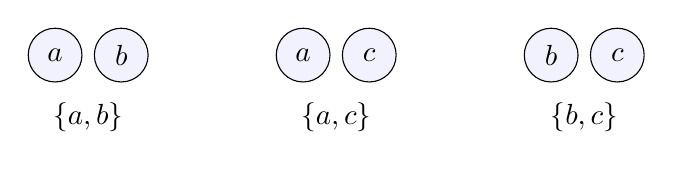
\begin{tikzpicture}[scale=1.05, transform shape]
\foreach \first/\second/\x in {a/b/0, a/c/3, b/c/6} {
    \node[draw, circle, fill=blue!5, minimum size=0.65cm] at (\x,0) {$\first$};
    \node[draw, circle, fill=blue!5, minimum size=0.65cm] at (\x+0.8,0) {$\second$};
    \node at (\x+0.4,-0.75) {$\{\first,\second\}$};
}
\end{tikzpicture}
\end{center}

\begin{theorembox}
The number of combinations without repetition of size \(k\) chosen from \(n\) distinct elements is
\[
\binom{n}{k}=\frac{n!}{k!(n-k)!}.
\]
\end{theorembox}

To see why, first count ordered selections without repetition. There are
\[
V(n,k)=\frac{n!}{(n-k)!}
\]
of them. But each unordered group of \(k\) elements can be ordered in \(k!\) ways. Therefore each combination has been counted \(k!\) times. Dividing by \(k!\) gives
\[
\frac{1}{k!}\cdot \frac{n!}{(n-k)!}=\frac{n!}{k!(n-k)!}.
\]

This division by \(k!\) is not a trick. It removes the internal orderings of the same selected group.

\begin{examplebox}
From six distinct books, choose three books to take on a trip. The order of choosing does not matter. The number of possible selections is
\[
\binom{6}{3}=\frac{6!}{3!3!}=20.
\]
\end{examplebox}

\begin{examplebox}
From the set \(\{1,2,3,4,5\}\), choose two numbers. The possible groups are not ordered, so \(\{1,4\}\) and \(\{4,1\}\) are the same group. The number of choices is
\[
\binom{5}{2}=10.
\]
\end{examplebox}

\begin{remarkbox}
Use combinations without repetition when order does not matter and no object may be selected more than once. Typical words are: choose, select, form a group, form a committee, pick a subset.
\end{remarkbox}

\section{Combinations with repetition}

The last basic scheme combines two ideas: order does not matter, but repetition is allowed. We select a group of objects, and the same kind of object may be selected more than once.

This scheme is less obvious than the previous ones, because the objects we are counting are not naturally written as ordered strings. A selection such as
\[
\{a,a,c\}
\]
contains two copies of \(a\), no copies of \(b\), and one copy of \(c\). The order in which we write these symbols is irrelevant.

\begin{definitionbox}
Let \(A\) be a finite set with \(n\) distinct elements. A combination with repetition of size \(k\) is a selection of \(k\) elements from \(A\), where elements may repeat and order does not matter.
\end{definitionbox}

For example, if
\[
A=\{a,b,c\}
\]
and we select \(2\) elements with repetition allowed, then the possible selections are
\[
\{a,a\},\quad \{a,b\},\quad \{a,c\},\quad \{b,b\},\quad \{b,c\},\quad \{c,c\}.
\]
The selections \(\{a,b\}\) and \(\{b,a\}\) are the same, because order does not matter.

\subsection*{Counting by multiplicities}

A useful way to count such selections is to record only how many times each element is chosen. If the elements are
\[
a_1,a_2,\ldots,a_n,
\]
then a selection of size \(k\) corresponds to a solution of
\[
x_1+x_2+\cdots+x_n=k,
\]
where each \(x_i\) is a non-negative integer. The number \(x_i\) tells how many times \(a_i\) is selected.

For example, if \(A=\{a,b,c\}\), then the selection \(\{a,a,c\}\) corresponds to
\[
x_a=2,\qquad x_b=0,\qquad x_c=1.
\]

\begin{theorembox}
The number of combinations with repetition of size \(k\) chosen from \(n\) distinct elements is
\[
\binom{n+k-1}{k}=\binom{n+k-1}{n-1}.
\]
\end{theorembox}

One way to understand the formula is the stars and bars method. Imagine \(k\) identical stars and \(n-1\) bars separating \(n\) boxes. The stars in the first box count how many times the first element is chosen, the stars in the second box count how many times the second element is chosen, and so on.

For example, with \(n=3\) and \(k=5\), the pattern
\[
\star\star\,|\,\star\,|\,\star\star
\]
represents
\[
x_1=2,
\qquad
x_2=1,
\qquad
x_3=2.
\]
Altogether there are \(k+n-1\) symbols: \(k\) stars and \(n-1\) bars. Choosing the positions of the stars determines the bars, and choosing the positions of the bars determines the stars. Therefore the number of patterns is
\[
\binom{k+n-1}{k}=\binom{k+n-1}{n-1}.
\]

\begin{examplebox}
A bag is to contain \(4\) candies chosen from \(3\) flavours: vanilla, chocolate, and strawberry. Repetition is allowed, and order does not matter. The number of possible bags is
\[
\binom{3+4-1}{4}=\binom{6}{4}=15.
\]
\end{examplebox}

\begin{examplebox}
How many non-negative integer solutions are there to
\[
x_1+x_2+x_3+x_4=7?
\]
This is the same as distributing \(7\) identical stars among \(4\) boxes. Hence the number of solutions is
\[
\binom{7+4-1}{7}=\binom{10}{7}=120.
\]
\end{examplebox}

\begin{remarkbox}
Use combinations with repetition when order does not matter and each type of object may be selected more than once. Typical words are: choose with repetition, distribute identical objects, non-negative integer solutions, multiset.
\end{remarkbox}

